\documentclass{article}

% Language setting
% Replace `english' with e.g. `spanish' to change the document language
\usepackage[english]{babel}

% Set page size and margins
% Replace `letterpaper' with `a4paper' for UK/EU standard size
\usepackage[letterpaper,top=2cm,bottom=2cm,left=3cm,right=3cm,marginparwidth=1.75cm]{geometry}

% Useful packages
\usepackage{amsmath}
\usepackage{graphicx}
\usepackage[colorlinks=true, allcolors=blue]{hyperref}

\title{Bayesian block decomposition.}
\author{Fyodor Sviridov}
\date{}
\begin{document}
\maketitle


\section{Introduction}

Implementation of Scargle's Bayesian Blocks algorithm is presented (\href{https://ui.adsabs.harvard.edu/abs/2013ApJ...764..167S/abstract}{Scargle et al. 2013}). This algorithm is used for optimal segmentation of data into blocks that characterize statistically significant variations. This algorithm has a certain elegance, as it is a great example of utilizing dynamic programming for a problem that cannot be solved in a brute straightforward way. The data may originate from different fields, but we used this method for time series analysis in astrophysics to determine the ranges of signal and background in light curves of gamma-ray bursts. Here, we will consider binned data, but the algorithm is not constrained to it. For further generalizations, we refer the reader to the original paper. 

\begin{figure}[h]
    \centering
    \begin{minipage}[b]{0.45\textwidth}
        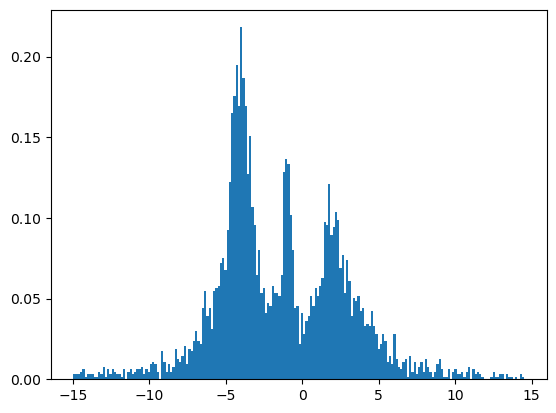
\includegraphics[width=\textwidth]{image1.png}
    \end{minipage}
    \hfill
    \begin{minipage}[b]{0.45\textwidth}
        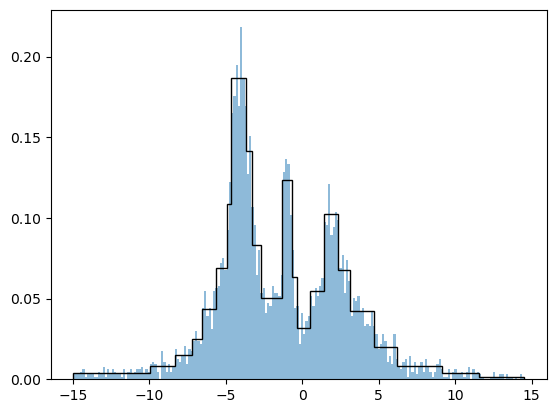
\includegraphics[width=\textwidth]{image2.png}
    \end{minipage}
    \caption{Bayesian block segmentation of an example dataset.}
    \label{fig:both_images}
\end{figure}

The task is to find some optimal segmentation by maximizing a certain criterion, referred to as a \textit{fitness function}. As we will see below, it's important that the total fitness function of a partition is block-additive. It must be the sum of the fitness functions of blocks, each evaluated only on the data within its respective block.
\begin{equation}
F[P]=\sum\limits_{k=1}^{N_{\text{blocks}}}f(B_k)
\end{equation}
where $F$ is the total fitness of the partition $P$ and $f(B_k)$ is the fitness of block $k$.

If there are $N$ cells (bins), then the number of all possible partitions of the data is $2^N$. For $N=100$ the optimization task becomes infeasible. However, due to the block-additivity of the fitness function, we can employ a dynamic programming algorithm, that is very similar to a mathematical proof by induction. We incrementally add one bin, and to solve the task for $n+1$ bins, we use saved information derived during previous steps ($\le n$). 

\section{Outline of the algorithm}
Let $P^{\text{opt}}(R)$ denote the optimal partition of the first $R$ bins. In the initial case $R=1$, the only possible partition is trivially optimal - a single block consisting of the first bin by itself. Once we have completed step $R$, having found the optimal partition $P^{\text{opt}}(R)$, we store the value of optimal fitness function in an array $\textbf{best}$ and the location of the last change point of the optimal partition is stored in an array $\textbf{last}$ (change point is the bin index where a block starts). To obtain the optimal partition  $P^{\text{opt}}(R+1)$, we consider partitions where the last block starts from  $r$ bin ($1\le r \le R+1$). Let fitness function of this last block be $F(r)$. Under the additivity assumption, the fitness of   $P^{\text{opt}}(R+1)$ is the sum of  $F(r)$ and the fitness of $P^{\text{opt}}(r-1)$, saved from previous steps in the array $\textbf{best}$.
\begin{equation}
    A(r) = F(r) + \begin{cases} 0,\quad r=1\\ \text{best}(r-1), \quad 2\le r\le R+1\end{cases}
\end{equation}

Optimal value maximizing $A(r)$ is computed:
$$ r^{\text{opt}}= \text{argmax}[A(r)] $$
After performing of all $N$ steps, we can obtain final optimal partition $P^{\text{opt}}(R+1)$, using the information contained in the array $\text{last}$, where we have stored the index $r^{\text{opt}}$ at each step. Indexes of change points in reverse order are
\begin{equation}
     i_1=\text{last}(N), \quad i_2=\text{last}(i_1-1), \quad i_3=\text{last}(i_2-1), \quad...
\end{equation}
The beauty of this algorithm is that it performs a complete search of the optimum in the space $2^N$ partitions in time of order $N^2$ 

\section{Fitness function}
\subsection{Piecewise constant model}
Now it is necessary to determine the fitness function of a certain model. For binned data, we will consider here \textit{piecewise constant model}. In many cases in astrophysics, we deal with the Poisson distribution. Therefore, the likelihood function of the $n$-th bin equals:
 \begin{equation}
     L_n=\frac{(\lambda W_n)^{N_n}\;e^{-\lambda W_n}}{N_n!}
 \end{equation}
where $N_n$ is the detected number of events in bin $n$, $\lambda$ is the actual event rate in counts per unit time, and $W_n$ is the bin width in time units. For a piecewise constant model, $\lambda$ remains constant inside the block. So the likelihood function of the block is:
\begin{equation}
    L^{(k)}(\lambda)=\prod_n L_n=\lambda^{N^{(k)}}\;e^{-\lambda W^{(k)}}
\end{equation}
where $N^{(k)}=\sum_n N_n$ and $W^{(k)}=\sum_n W_n$ are the total number of counts and the block width, respectively. Here, we are omitting a constant term that depends only on the full sample, is irrelevant to the fitness when summed over all blocks. The log-likelihood is 
\begin{equation}
    \ln L^{(k)}(\lambda)=N^{(k)}\ln\lambda-\lambda W^{(k)}
\end{equation}
The maximum is reached when $\lambda_{\text{max}}=N^{(k)}/W^{(k)}$, which has the meaning of the average count rate in the block. The maximum value of the log-likelihood is the fitness function of the block:
\begin{equation}
f^{(k)}=N^{(k)}\ln\frac{N^{(k)}}{W^{(k)}}-N^{(k)}
\end{equation}

\subsection{Number of blocks}
But under the derivation above, we have not considered how many blocks there are in a partition. It remains to implicitly include a parameter in the fitness that corresponds to the number of blocks in a model. For this purpose, we need to multiply the likelihood by a prior distribution for the number of blocks:
\begin{equation}
P(N_{\text{blocks}})=p_0\;\gamma^{-N_{\text{blocks}}}
\end{equation}
where $p_0$ is a normalization constant,  $0\le N_{\text{blocks}}\le N$ and $\gamma\ge 1$. By choosing this prior it is much more likely that $N_{\text{blocks}}\ll N$, as we assume in advance. Then, the posterior probability (the total fitness of a partition $F[P]$) equals:
\begin{equation}
    F[P](\vec{\lambda}, N_{\text{blocks}})=\prod\limits_{k=1}^{N_{\text{blocks}}}\left[L^{(k)}(\lambda_k)\right]\cdot P(N_{\text{blocks}})
\end{equation}
And :
\begin{equation}
    \ln F[P]=\sum\limits_{k=1}^{N_{\text{blocks}}}\ln L^{(k)}-N_{\text{blocks}}\ln\gamma=
\end{equation}
\begin{equation*}
=\sum\limits_{k=1}^{N_{\text{blocks}}}\left(\ln L^{(k)}-\ln\gamma\right)
\end{equation*}
So maximizing it over $\vec{\lambda}$ leads us to the final fitness function of a partition: 
\begin{equation}
    \ln F[P] = \sum\limits_{k=1}^{N_{\text{blocks}}}f^{(k)} 
\end{equation}
\begin{equation}
f^{(k)}=\left(N^{(k)}\ln\frac{N^{(k)}}{W^{(k)}}-N^{(k)} \right)\ - \text{ncp\_prior}
\end{equation}
where $f^{(k)}$ is the fitness function of k-th block, $N^{(k)}=\sum_n N_n$ and $W^{(k)}=\sum_n W_n$ are the total number of counts and the block width, respectively. $\text{ncp\_prior} \equiv \log\gamma$ is the parameter from 0 to $+\infty$, that controls the number of blocks, with a zero value corresponding to $N_{\text{blocks}}=N$, while a large value corresponds to one or just few blocks covering all data.

\subsection{Piecewise linear model}
A derivation for the piecewise linear fitness function follows similar lines, we need only to introduce a new inclined parameter $a$. In this model, data can be changed inside a block:
\begin{equation}
    \lambda \rightarrow\lambda(1+a(n - n_i)) = \lambda(1+a\Delta n)
\end{equation}
where $n$ is the bin number, $n_i$ is the first bin number of some block.
Log-likelihood function of the k-th block equals
\begin{equation}
    \ln L^{(k)} =  N^{(k)}\ln\lambda + \sum\limits_{n=n_i}^{n_f} N_n\ln[(1+a\Delta n)W_n]-\sum\limits_{n=n_i}^{n_f}\lambda (1+a\Delta n)W_n
\end{equation}
For solving the piecewise constant model, we previously omitted the second term, but now it is necessary due to its dependency on the new parameter. From $d/d\lambda \ln L^{(k)} = 0$, we can find $\lambda_{\text{max}}$

\begin{equation}
\lambda_{max}=\frac{N^{(k)}}{\sum\limits_{n} (1+a\Delta n)W_n}
\end{equation}
And thereby,
\begin{equation}
    \ln L^{(k)}(\lambda_{max}, a) = N^{(k)}\left(\ln\frac{N^{(k)}}{\sum\limits_{n} (1+a\Delta n)W_n} - 1\right) + \sum\limits_{n} N_n\ln[(1+a\Delta n)W_n
\end{equation}

The maximum value of this equation defines the fitness function of k-th block (omitting the subtraction of $\text{ncp\_prior}$). If $a=0$ we get the already well-known function for the piecewise constant model.
There is a lower bound on the parameter $a$, arising from the requirement that expectation of $\lambda(1+a\Delta n)$ events should be positive.
$$a>-1/N$$

\section{References}
[1] Scargle, J et al. (2013), ApJ, Studies in Astronomical Time Series Analysis. VI. Bayesian Block Representations, 764, 2, 167. \href{https://ui.adsabs.harvard.edu/abs/2013ApJ...764..167S/abstract}{doi:10.1088/0004-637X/764/2/167}

\end{document}
